\begin{abstract}
Spatial perturbation assays preserve tissue architecture, but observed
neighbor responses conflate stable tissue context with
perturbation-conditioned effects. We construct Pre--Post Perturbation Pairing
(\ppp), an audited matched-control pseudo-target benchmark, and \methodname{},
a predictive decomposition that first estimates context-explainable response
and then models the residual conditioned on a direct-effect profile and sender
region. On a fully disjoint 1,342/837/928-graph train/validation/test split,
\methodname{} increases pooled Ring Pearson from 0.3626 to 0.4111; the mean
graph-paired lift is $+0.0532$ (95\% CI, 0.0474--0.0586). Context-only and full
models attain predictive $R^2$ values of 0.3712 and 0.4669, corresponding to an
incremental partial $R^2$ of 0.1521 (0.1476--0.1559). Gene-disjoint and
no-expression matching retain positive Ring lift, whereas removing spatial
matching does not, indicating that the signal is not explained solely by
expression overlap but depends on spatially matched controls. Factorial
controls show contributions from both direct-effect profile identity and sender
location, while randomized communication scores have no measurable effect.
Across five guide-OOD folds, assay-matched spatial seeds improve Ring Pearson
from 0.4400 to 0.4619, whereas external scRNA-derived seeds underperform the
zero-seed baseline, identifying cross-assay seed transfer as the current
end-to-end bottleneck. On a formal three-way selector split, \methodname{}
preserves target-qualified rate at 0.6944 while reducing mean spillover by
12.0\% and absolute burden by 0.1244 (0.0559--0.1926). These results support
context-dominated global fields, perturbation-structured local organization,
and modest retrospective lower-burden prioritization rather than causal or
clinical prediction.
\end{abstract}

\begin{CCSXML}
<ccs2012>
 <concept>
  <concept_id>10010147.10010257</concept_id>
  <concept_desc>Computing methodologies~Machine learning</concept_desc>
  <concept_significance>500</concept_significance>
 </concept>
 <concept>
  <concept_id>10002950.10003714.10003715</concept_id>
  <concept_desc>Mathematics of computing~Graph algorithms</concept_desc>
  <concept_significance>300</concept_significance>
 </concept>
</ccs2012>
\end{CCSXML}
\ccsdesc[500]{Computing methodologies~Machine learning}
\ccsdesc[300]{Mathematics of computing~Graph algorithms}
\keywords{spatial functional genomics, perturbation response, spatial
transcriptomics, graph neural networks, perturbation prioritization}

\maketitle

\section{Introduction}
Spatial functional genomics places genetic perturbations within intact tissue
and measures molecular changes in situ
\citep{dhainaut2022spatialcrispr,binan2025perturbfish,shen2026spatialperturbseq}.
Unlike dissociated Perturb-seq, these assays can reveal whether a local
intervention remains confined to its intended niche or reorganizes distant and
off-program responses. Their cost and sparsity, however, make it impractical to
measure every perturbation in every tissue context. Predictive models could
help prioritize experiments, but only if the spatial signal they use is
genuinely perturbation-conditioned.

This requirement creates an evaluation problem. High correlation between
predicted and observed neighbor expression can arise from reconstructing stable
anatomy, cell state, or local composition rather than learning perturbation
propagation. Spatial variance and multiview models already show that intrinsic
and environmental components explain substantial spatial expression variation
\citep{arnol2019svca,tanevski2022misty,fischer2023ncem}. In a perturbation
assay, the measured neighbor field therefore mixes a context-explainable
component with a weaker perturbation-conditioned component, and flat
cell--gene correlation can obscure their distinction.

We ask four linked scientific questions: how much observed neighbor response is
predictable from tissue context; where perturbation-conditioned signal remains
after accounting for context; whether that residual transfers across regions,
guides, and assays; and whether predicted fields can prioritize perturbations
that preserve a requested local response while reducing collateral burden.
On the fully separated spatial split, context-only and full models reach pooled
Ring Pearson 0.3626 and 0.4111, with mean graph-paired lift $+0.0532$.
Predictive $R^2$ increases from 0.3712 to 0.4669, corresponding to partial
$R^2=0.1521$ conditional on context. Matching-decoupling experiments preserve
positive lift after removing expression overlap, but not after removing spatial
matching. Across five held-out-guide folds, assay-matched spatial seeds provide
a modest positive lift, whereas external scRNA seeds fail to transfer. A
validation-frozen selector finally preserves target qualification and reduces
held-out burden by 12.0\%.

These results support a narrower conclusion than ``the full field is
predictable'': spatial perturbation fields are \emph{globally
context-dominated but locally perturbation-structured}. We contribute
(1) an independently validated predictive decomposition with effect-size and
partial-$R^2$ estimates; (2) an audited \ppp benchmark with matching-decoupling
and spatial-scale analyses; (3) a parsimonious response-field model with
conditional propagation-transfer and cross-assay failure analyses; and
(4) a formal retrospective perturbation-prioritization task that separates
confirmatory effects from exploratory cases.

\section{Related Work}
\textbf{Context in spatial molecular data.}
SVCA decomposes spatial molecular variation into intrinsic, environmental, and
cell--cell interaction components \citep{arnol2019svca}; MISTy models
intraview, juxtaview, and paraview effects
\citep{tanevski2022misty}; and NCEM predicts gene expression from a spatial
graph and niche composition \citep{fischer2023ncem}. These methods motivate our
context audit, but do not condition a cell-resolved perturbation-response field
on a direct-effect profile.

\textbf{Perturbation models.}
Dissociated-cell methods learn conditional translations, transport maps, gene
graphs, or disentangled representations
\citep{lotfollahi2019scgen,Lotfollahi2023,bunne2023cellot,roohani2023gears,piran2024biolord}.
They provide candidate direct-effect profiles but remove the tissue graph.
Spatial functional assays restore that graph
\citep{dhainaut2022spatialcrispr,binan2025perturbfish,shen2026spatialperturbseq}.
SpatialProp, Celcomen, and CONCERT connect perturbations to spatial context
\citep{spatialprop2025,celcomen2026,concert2025}. \methodname{} targets a
specific interface: given a sender region and measured or predicted
direct-effect profile, estimate a signed receiver field and quantify lift over
context and seed nulls.

\begin{figure*}[t]
\centering
\fbox{\parbox[t][1.20in][t]{0.298\textwidth}{
\textbf{A. Observed field is mixed}\par\smallskip
An intact-tissue response contains stable anatomy and local composition
together with a weaker perturbation-conditioned component.\par\medskip
\centering
$\Delta^{\mathrm{PPP}}\approx C_{\mathrm{context}}+
R_{\mathrm{perturbation}}$
}}
\hfill
\fbox{\parbox[t][1.20in][t]{0.298\textwidth}{
\textbf{B. Predictive separation}\par\smallskip
\methodname{} first predicts context-explainable response, then routes a
direct-effect profile from sender cells to receivers.\par\medskip
\centering
$G,X,c,p\rightarrow\widehat C$\par
$G,X,a,d,e\rightarrow\widehat R$\par
$\widehat\Delta=\widehat C+\widehat R$
}}
\hfill
\fbox{\parbox[t][1.20in][t]{0.298\textwidth}{
\textbf{C. Scientific use}\par\smallskip
Predicted fields define local target utility $U$ and collateral spatial burden
$S$. Candidate perturbations are compared under target retention.\par\medskip
\centering
$\min_a\widehat S(a)$ s.t.\ $\widehat U(a)\geq\tau$
}}
\caption{\textbf{Scientific problem and analysis framework.}
The core model uses context prediction and direct-effect-conditioned residual
routing. The separation is predictive, not an identifiable causal
decomposition. Reference-ST and cached communication priors are evaluated only
as optional diagnostics.}
\label{fig:main_framework}
\Description{Three-panel conceptual diagram showing a mixed spatial response,
predictive context and perturbation-conditioned components, and
target-constrained perturbation prioritization.}
\end{figure*}

\section{Problem and Benchmark}
\label{sec:data_construction}
\subsection{Spatial Response-Field Task}
Let $G=(V,E)$ be a local tissue graph, $X$ its matched pre-perturbation
expression, $a_i$ a direct-effect-cell indicator, and $d_i$ a measured or
predicted direct-effect profile. The task is to predict the signed
post-minus-pre response for every cell:
\[
\Delta_i=X_i^{\mathrm{post}}-X_i,\qquad i\in V.
\]
We distinguish direct-effect cells ($a_i=1$) from receiver cells ($a_i=0$),
and evaluate receiver responses both over all cell--gene pairs and after
aggregation into three distance-ranked rings. The task is predictive: neither
the target nor the model identifies a causal intercellular communication path.

\subsection{Pre--Post Perturbation Pairing}
\label{sec:ppp_construction}
Spatial Perturb-seq does not observe the same cell before and after
perturbation. \ppp constructs a pseudo-pre-state for each perturbed anchor.
It forms a 64-cell post patch, ranks control-like anchors using spatial
distance, center-expression similarity, and patch-expression similarity,
softly aligns the top $K=3$ controls to the post coordinate frame, and
aggregates their post-minus-pre deltas with matching-score weights. A nominal
cell-type-composition channel is present in the implementation, but all coarse
labels in the reported cache map to one effective ID and the channel is
constant.

\begin{figure*}[t]
\centering
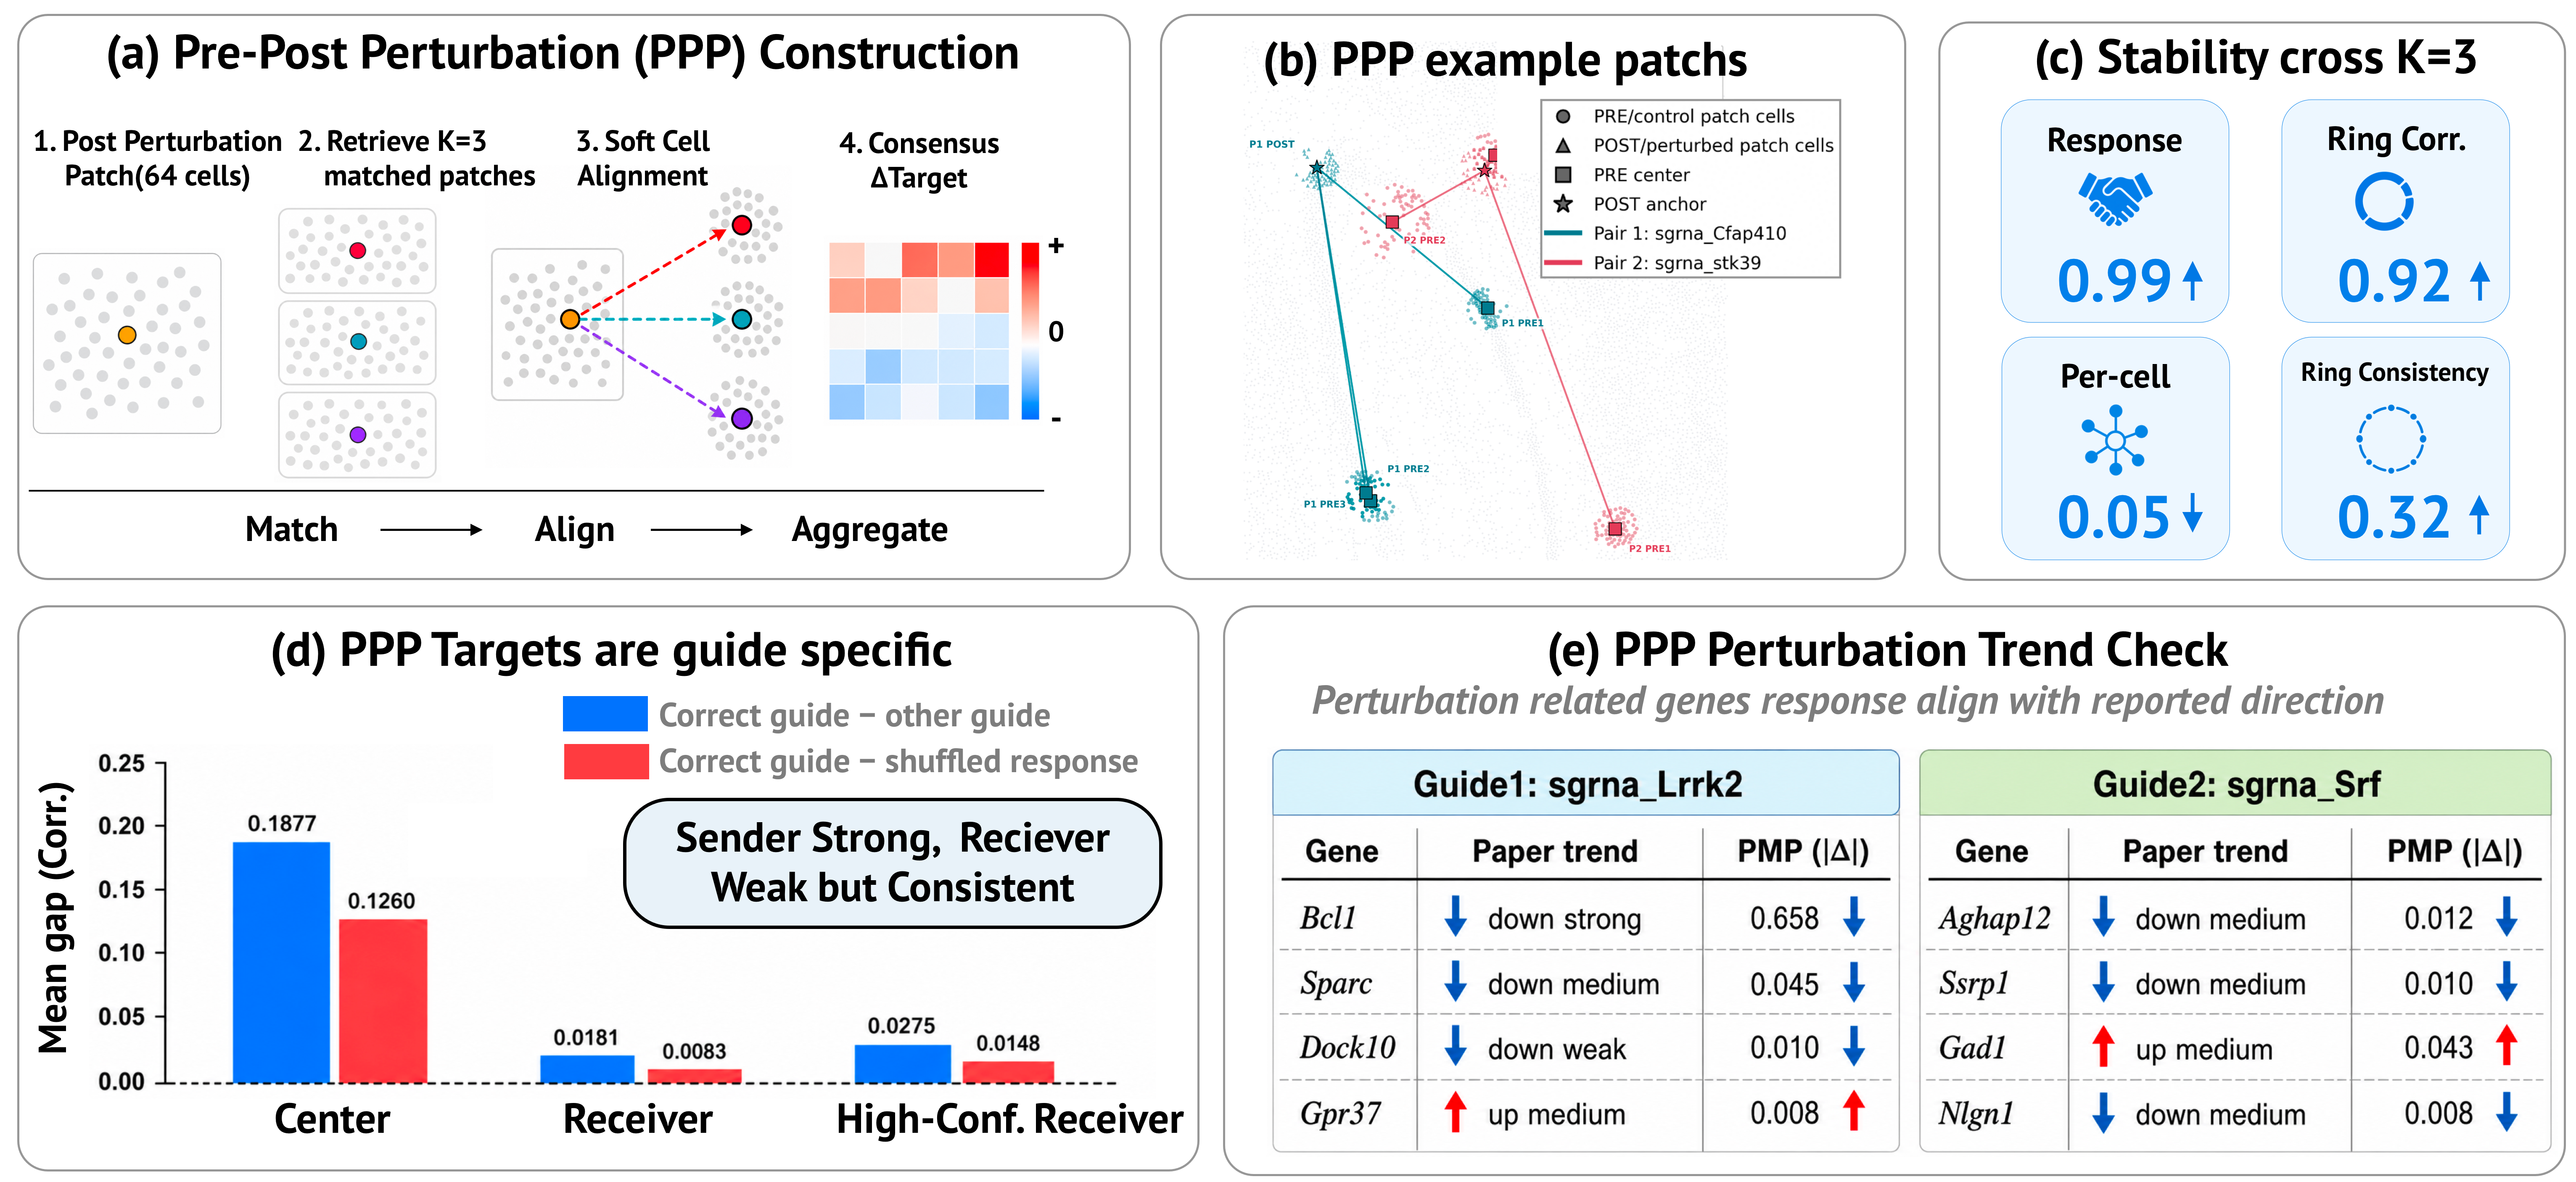
\includegraphics[width=0.88\linewidth]{pair_2.png}
\caption{\textbf{\ppp construction and audit.}
(a) Each 64-cell post-perturbation patch is matched to $K=3$ control patches,
softly aligned, and aggregated into a consensus response pseudo-target.
(b) Example matched patches. (c--e) Multi-control stability and guide-aware
nulls. Consensus/ring correlations are 0.944/0.923; own-guide alignment exceeds
wrong-guide and target-shuffled alignment at direct-effect and receiver cells.
Expression-decoupled, gene-disjoint, channel-removal, and no-spatial audits are
reported in \Cref{tab:confirmatory_analysis}. They support robustness to
expression overlap, while the no-spatial variant shows that \ppp still depends
on spatially matched controls.}
\label{fig:data_pair}
\Description{Five-panel PPP diagram showing matched-control construction,
aligned control and post patches, target stability, and guide-aware nulls.}
\end{figure*}

Spatial partitions are assigned before matching, preventing held-out post
anchors or matched controls from entering training. Consensus and ring
consistency are 0.944 and 0.923. Across 512 genes, own-guide versus wrong-guide
alignment is 0.317 versus 0.129 at the center, 0.022 versus 0.004 in
high-confidence receivers, and 0.029 versus 0.001 over all receivers. Because
matching and model inputs partly overlap, \ppp is treated as a stable,
guide-consistent pseudo-target rather than a causal counterfactual.

\subsection{Splits, Metrics, and Scope}
We use two evaluation regimes. The original exact-task comparison uses all
development graphs and 928 block-held-out test graphs so that fourteen
implemented alternatives can be compared on the same task. The strict
confirmatory split uses 1,342 training, 837 validation, and 928 test graphs from
fully separated spatial regions. All scientific effect sizes, robustness
audits, and formal selector results use the strict split.

We report Neighbor Pearson over receiver cell--gene pairs, receiver-centered
Pearson after subtracting each receiver profile mean, Ring Pearson over
distance-ring gene summaries, and receiver MAE. Pooled Ring Pearson concatenates
ring summaries across test graphs. Graph-paired Ring lift first computes
full-minus-context change within each graph and then averages; it is therefore
not the difference of pooled correlations. Predictive $R^2$ is computed from
held-out squared error, and incremental partial
$R^2=1-\mathrm{SSE}_{\mathrm{full}}/\mathrm{SSE}_{\mathrm{context}}$.
Guide-cluster bootstrap retains all graphs from each sampled guide;
spatial-cluster bootstrap retains all values from sampled test clusters.
Selector intervals resample the 36 target specifications.

\section{Method}
\label{sec:method}
\subsection{Task and Predictive Decomposition}
\label{sec:method_task}
Each graph has matched-control expression $x_i\in\mathbb R^G$, nominal cell
state $c_i$, relative position $p_i$, sender-relative geometry $g_i$,
direct-effect indicator $a_i$, and direct-effect profile $d_i$ when $a_i=1$.
Edge features $e_{ij}$ encode relative geometry, nominal state pairs, and an
optional communication-compatibility score. \methodname{} predicts
\begin{equation}
\widehat\Delta_i=\widehat C_i+\widehat R_i,\qquad
\widehat X_i^{\mathrm{post}}=x_i+\widehat\Delta_i ,
\label{eq:predictive_decomposition}
\end{equation}
Here $\widehat C_i$ is context-explainable response. The second term,
$\widehat R_i$, is the perturbation-conditioned residual. This predictive
decomposition does not identify a causal communication pathway or imply that
every residual response was transmitted from the direct-effect cells.

\subsection{Context-Explainable Component}
\label{sec:method_context}
The context model is trained with direct-effect indicators and profiles masked:
\begin{equation}
\widehat C_i=f_{\mathrm{context}}(x,c,p,e;\,a=0,d=0),
\qquad
R_i^\star=\Delta_i^{\mathrm{PPP}}-\widehat C_i .
\label{eq:context_residual}
\end{equation}
It is trained first and frozen before residual-model optimization. The residual
target $R_i^\star$ therefore asks the second stage to model response remaining
after the implemented context predictor, rather than the full
context-dominated field.

\subsection{Direct-Effect-Conditioned Residual Routing}
\label{sec:method_residual}
The model embeds baseline and spatial features, then initializes separate
receiver and direct-effect states:
\begin{equation}
\begin{aligned}
h_i&=\phi_x(x_i)+\phi_c(c_i)+\phi_p(p_i)+\phi_g(g_i),\\
b_i&=\phi_N(h_i),\qquad n_i^0=0,\\
u_i&=a_i\phi_D([h_i,d_i,g_i]).
\end{aligned}
\label{eq:state_initialization}
\end{equation}
Thus $u_i$ is nonzero only at direct-effect cells, and receivers never directly
observe $d_i$. For each implemented propagation layer, the code retains only
edges whose source is a direct-effect cell and destination is a receiver:
\begin{equation}
\begin{aligned}
z_{ij}^{\ell}
&=\sigma\!\left(
\phi_a([u_i,b_j,n_j^\ell,e_{ij}])+w_{\mathrm{comm}}q_{ij}
\right),\\
\mu_{ij}^{\ell}
&=z_{ij}^{\ell}\phi_\mu([u_i,b_j,e_{ij}]),\\
n_j^{\ell+1}
&=\operatorname{LN}\!\left(n_j^\ell+
\sum_{\substack{i:(i,j)\in E\\a_i=1}}\mu_{ij}^{\ell}\right)
+\phi_u([n_j^\ell,b_j]).
\end{aligned}
\label{eq:directed_message_passing}
\end{equation}
Direct-effect states remain fixed; there is no receiver-to-receiver message
path in the core implementation. A receiver head decodes $\widehat R_j$ from
$b_j$, $n_j^L$, and the graph-level sender summary. Communication scores are
optional gate biases. Randomizing cached scores leaves Ring Pearson unchanged
(0.4574 versus 0.4575), so we do not attribute the measured lift to this prior.

\subsection{Training and Inference}
\label{sec:training_inference}
The residual model is optimized with the implemented objective
\begin{equation}
\mathcal L_{\mathrm{prop}}
=\mathcal L_{\mathrm{neighbor}}
+0.3\mathcal L_{\mathrm{ring}}
+0.3\mathcal L_{\mathrm{post}}
+0.1\mathcal L_{\mathrm{rank}} .
\label{eq:training_objective}
\end{equation}
$\mathcal L_{\mathrm{neighbor}}$ is Huber loss over high-confidence receivers;
$\mathcal L_{\mathrm{ring}}$ supervises three ring-level response summaries;
$\mathcal L_{\mathrm{post}}$ reconstructs post-state expression; and
$\mathcal L_{\mathrm{rank}}$ preserves within-graph gene-response ordering.
Direct-effect-cell loss has weight zero in the reported propagation setting so
that the easier sender task does not dominate receiver learning. At inference,
$d_i$ is either measured in the spatial assay or supplied by an external
direct-effect assay, then routed through the frozen graph model.

The exact-task comparison also evaluates an optional distance-aware response
refinement, reported as \methodname{}-Refine. An unperturbed reference-ST
adapter yields paired Ring gains of only $+0.0009$, $+0.0002$, and $+0.0032$
at 10\%, 25\%, and 50\% paired-data fractions, with approximately $+0.0005$ at
full data. We exclude it from the core definition and report it only as a
negative appendix diagnostic.

\subsection{Spatially Constrained Perturbation Prioritization}
\label{sec:intervention_method}
For action $a$, target program $t$, and requested ring $r$, utility
$U(a;t,r)$ is the signed target-program response. Collateral burden is
\begin{equation}
S(a;t,r)=\lambda_{\mathrm{far}}S_{\mathrm{far}}
+\lambda_{\mathrm{off}}S_{\mathrm{off}}
+\lambda_{\mathrm{undes}}S_{\mathrm{undes}},
\label{eq:burden}
\end{equation}
combining far-field target response, off-program response, and response in
validation-defined undesirable programs. The selector is
\begin{equation}
a^\star=\arg\min_{a:\widehat U(a)\geq\tau}\widehat S(a).
\label{eq:selector}
\end{equation}
Program definitions, weights, utility threshold, and operating point are
selected on validation data and frozen. Observed test fields are used only for
evaluation. This formal analysis is separate from the exploratory post-hoc
case discovery.

\section{Experiments}
\label{sec:experiments}
\subsection{Evaluation Design}
The primary benchmark is mouse-brain Spatial Perturb-seq. The complete
exact-task suite is implemented on the original full-development comparison
split; all perturbation-specific effect estimates are independently
re-estimated on the stricter three-way spatial split. Five grouped guide-out
folds assign every guide to test once. Observed spatial seeds evaluate
conditional propagation transfer, while companion scRNA seeds test the
end-to-end cross-assay interface. Supporting analyses use a controlled
ligand--receptor benchmark, Perturb-map, and Perturb-FISH. Metrics and
resampling units follow \Cref{sec:data_construction}; detailed source tables,
per-fold results, and complete gene distributions are in the appendix.

\subsection{Main Spatial Response-Field Prediction}
\label{sec:main_prediction}
\begin{figure*}[t]
\centering
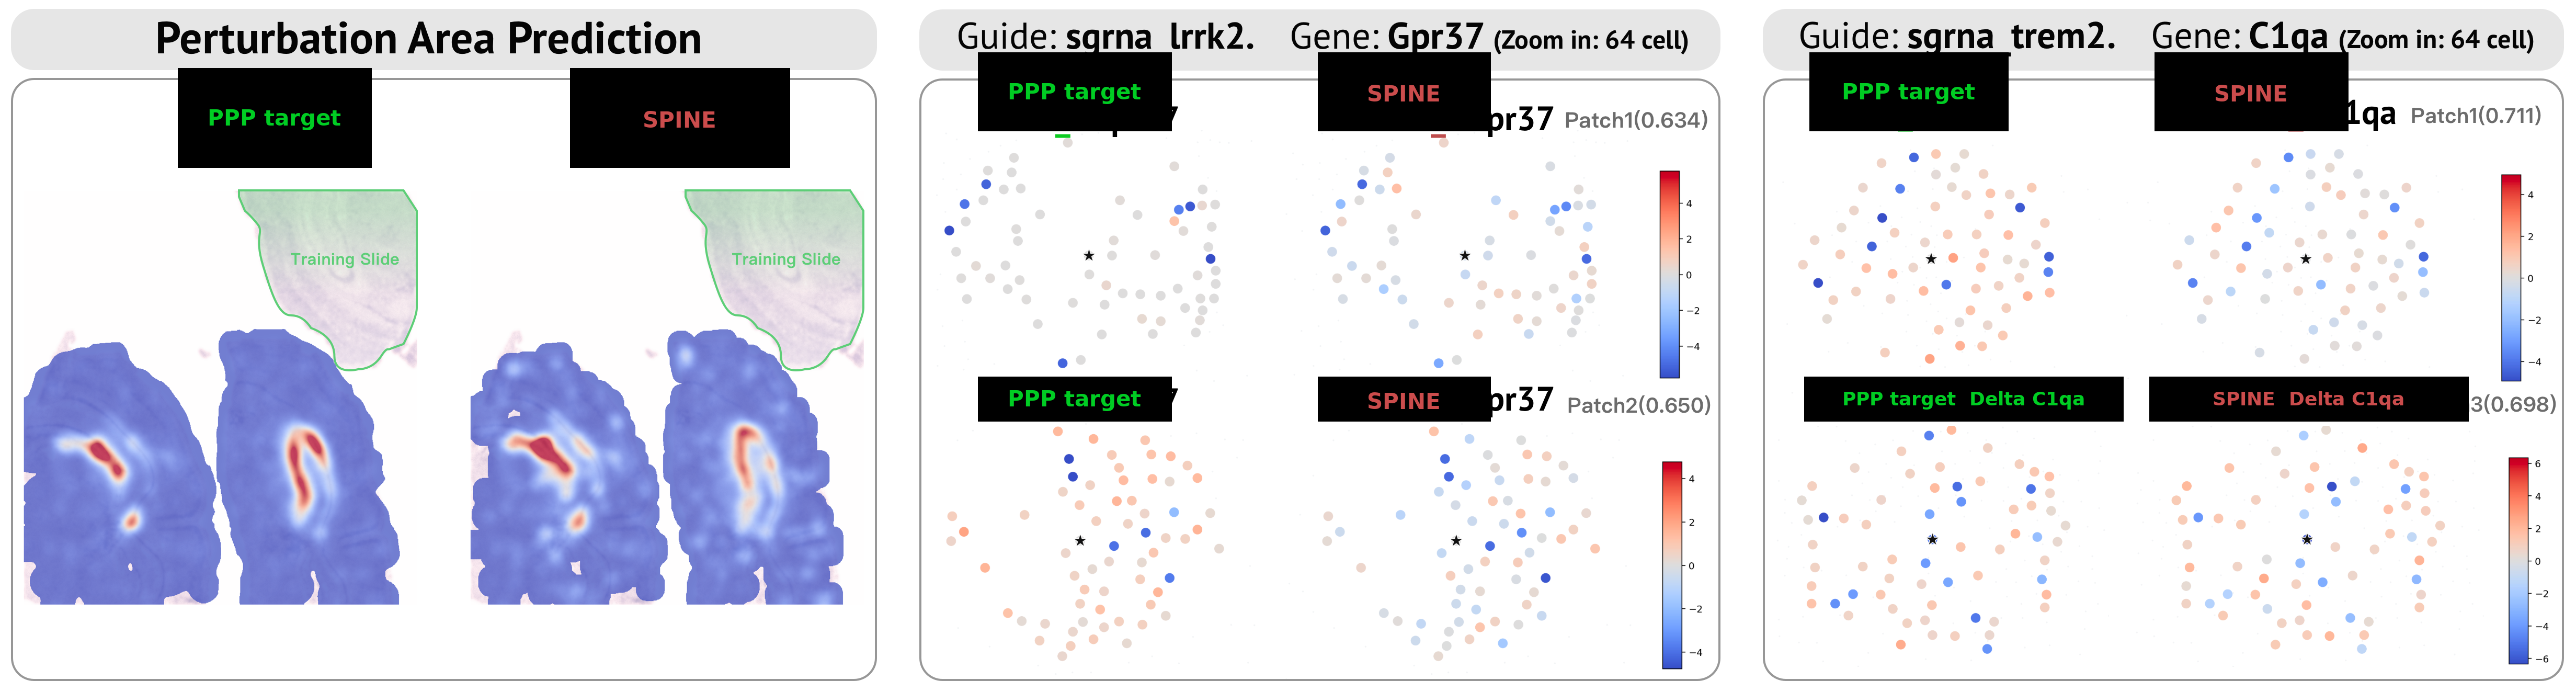
\includegraphics[width=0.94\linewidth]{main_exp.png}
\caption{\textbf{Qualitative response-field predictions on the held-out Spatial
Perturb-seq test region.}
The left panel compares the whole-region \ppp pseudo-target and \methodname{}
prediction. The remaining panels show representative 64-cell neighborhoods for
\textit{Gpr37} under sgRNA-\textit{Lrrk2} and \textit{C1qa} under
sgRNA-\textit{Trem2}. Colors denote signed response deltas and stars mark
direct-effect cells. Quantitative conclusions use all 928 test graphs and all
512 genes.}
\label{fig:main_exp_kdd}
\Description{Whole-region and local spatial maps comparing PPP pseudo-targets
with SPINE predictions for Gpr37 under Lrrk2 perturbation and C1qa under Trem2
perturbation.}
\end{figure*}

\begin{table*}[t]
\centering
\scriptsize
\caption{\textbf{Exact-task comparison on the original full-development block-held-out benchmark.} This comparison uses the original full-development benchmark. All confirmatory effect estimates use the strict 1,342/837/928 split in \Cref{tab:confirmatory_analysis}.}
\label{tab:exact_task_main}
\setlength{\tabcolsep}{5.2pt}
\begin{tabular}{llrrrr}
\toprule
Group & Method & Neighbor $\uparrow$ & Centered $\uparrow$ & Ring $\uparrow$ & MAE $\downarrow$ \\
\midrule
Trivial & Zero-delta & 0.00000 & 0.00000 & 0.00000 & 0.45344 \\
Statistical & Guide $\times$ cell-type $\times$ ring mean & 0.00714 & -0.00045 & 0.01731 & 0.46752 \\
Retrieval & Nearest patch transfer & 0.00012 & -0.00104 & 0.00960 & 0.61186 \\
Direct/radial & Direct-effect diffusion & 0.00616 & 0.00028 & 0.01434 & 0.45912 \\
 & CCC-gated linear & -0.00191 & 0.00316 & 0.00052 & 0.50968 \\
 & Direct-effect broadcast & 0.01572 & -0.00000 & 0.05311 & 0.83524 \\
 & Fixed-decay broadcast & 0.01526 & 0.00320 & 0.05306 & 0.59406 \\
 & Learned radial ridge & 0.02293 & -0.00150 & 0.06547 & 0.52651 \\
Supervised & Elastic-net & 0.56953 & 0.59375 & 0.39101 & 0.42737 \\
 & Patch MLP & 0.27241 & 0.44395 & 0.08649 & 0.67715 \\
 & Graph Transformer & 0.54306 & 0.56345 & 0.39277 & 0.45970 \\
 & Neural CCC--GNN & 0.54343 & 0.56475 & 0.39249 & 0.46392 \\
SPINE & \textbf{\methodname{}-Core} & 0.68410 & 0.71701 & 0.45204 & 0.40939 \\
 & \textbf{\methodname{}-Refine} & 0.68443 & 0.71566 & 0.45722 & 0.40762 \\
\bottomrule
\end{tabular}
\end{table*}


\Cref{fig:main_exp_kdd} shows that the model produces signed local and
whole-region fields rather than only patch summaries. On the original
exact-task comparison split, \methodname{}-Core reaches Neighbor/Ring Pearson
0.684/0.452, and optional refinement changes Ring Pearson to 0.457 while
leaving Neighbor Pearson unchanged (\Cref{tab:exact_task_main}). It outperforms
the implemented statistical, retrieval, radial, linear, patch, and generic
graph alternatives on this common output. Because this split uses the full
development set, it is a model-comparison result only; perturbation-specific
effect size is evaluated on the strict split below.

\subsection{Signal Decomposition and Benchmark Robustness}
\label{sec:signal_robustness}
\begin{table*}[t]
\centering
\scriptsize
\caption{\textbf{Confirmatory signal decomposition, benchmark decoupling, and transfer diagnostics.} Panels A, C, and E use the strict three-way spatial split. Pooled Ring correlation and graph-paired lift are different estimands. Partial $R^2=1-\mathrm{SSE}_{\mathrm{full}}/\mathrm{SSE}_{\mathrm{context}}$.}
\label{tab:confirmatory_analysis}
\setlength{\tabcolsep}{3.0pt}
\begin{minipage}[t]{0.49\textwidth}
\centering
\textbf{A. Independent spatial split and predictive variance}\\[-0.2em]
\resizebox{\linewidth}{!}{%
\begin{tabular}{lrrrr}
\toprule
Metric & Context & Full & Effect & 95\% CI \\
\midrule
Pooled Ring Pearson & 0.3626 & 0.4111 & -- & -- \\
Mean graph-paired Ring lift & -- & -- & +0.0532 & [0.0474, 0.0586] \\
Predictive $R^2$ & 0.3712 & 0.4669 & partial $R^2$ = 0.1521 & [0.1476, 0.1559] \\
\bottomrule
\end{tabular}
}
\medskip
\textbf{B. Direct-effect profile/location factorial}\\[-0.2em]
\begin{tabular}{lr}
\toprule
Input control & Ring Pearson \\
\midrule
Correct profile + correct region & 0.4574 \\
Shuffled profile + correct region & 0.4056 \\
Correct profile + relocated region & 0.4314 \\
Random profile + random region & 0.4135 \\
Correct profile + randomized CCC & 0.4575 \\
\bottomrule
\end{tabular}
\medskip
\textbf{C. PPP decoupling}\\[-0.2em]
\begin{tabular}{lrr}
\toprule
PPP construction & Paired lift & 95\% CI \\
\midrule
Gene-disjoint matching/output genes & +0.0257 & [0.0215, 0.0302] \\
No center-expression matching & +0.0281 & [0.0244, 0.0319] \\
No patch-expression matching & +0.0263 & [0.0226, 0.0300] \\
Strict no-expression matching & +0.0128 & [0.0088, 0.0166] \\
No spatial matching & +0.0025 & [-0.0022, 0.0066] \\
\bottomrule
\end{tabular}
\end{minipage}
\hfill
\begin{minipage}[t]{0.49\textwidth}
\centering
\textbf{D. Five-fold guide-OOD seed transfer}\\[-0.2em]
\resizebox{\linewidth}{!}{%
\begin{tabular}{lrrrr}
\toprule
Seed source & Zero & Seed & Difference & Direction \\
\midrule
Assay-matched spatial seed & 0.4400 & 0.4619 & +0.0220 & 5/5 positive \\
External scRNA seed & 0.4400 & 0.4130 & -0.0270 & 5/5 below zero-seed \\
\bottomrule
\end{tabular}
}
\medskip
\textbf{E. Patch-scale sensitivity}\\[-0.2em]
\resizebox{\linewidth}{!}{%
\begin{tabular}{lrrr}
\toprule
Patch and median radius & Context & Full & Paired lift \\
\midrule
32 cells; median radius 67.83\,$\mu$m & 0.2775 & 0.3142 & +0.0430 \\
64 cells; median radius 98.18\,$\mu$m & 0.3626 & 0.4111 & +0.0532 \\
100 cells; median radius 125.79\,$\mu$m & 0.4826 & 0.4722 & -0.0077 \\
128 cells; median radius 144.60\,$\mu$m & 0.4739 & 0.4470 & -0.0246 \\
\bottomrule
\end{tabular}
}
\medskip
\parbox{0.96\linewidth}{\raggedright \textit{Reading.} Expression-decoupled variants retain positive lift, whereas no-spatial matching does not. Assay-matched spatial seeds improve all five guide-OOD folds; external scRNA seeds underperform zero seed in all five.}
\end{minipage}
\end{table*}


\textbf{Independent validation.}
With train/validation/test regions fully separated, context and full models
reach pooled Ring Pearson 0.3626 and 0.4111. The mean graph-paired lift is
$+0.0532$ (guide-cluster bootstrap 95\% CI, 0.0474--0.0586). The pooled
difference and paired lift are not algebraically identical because they
aggregate at different levels.

\textbf{Predictive variance decomposition.}
Context and full models explain $R^2=0.3712$ and 0.4669 of receiver variation,
respectively. The resulting partial $R^2=0.1521$ (spatial-cluster bootstrap
95\% CI, 0.1476--0.1559) means that perturbation conditioning explains 15.2\%
of the squared-error variance remaining after context prediction. This is a
predictive, not causal, variance decomposition.

\textbf{\ppp matching decoupling.}
Positive paired Ring lift survives disjoint matching and output genes
($+0.0257$), removal of center expression ($+0.0281$), removal of
patch expression ($+0.0263$), and strict no-expression matching
($+0.0128$). Removing spatial matching reduces lift to $+0.0025$, with a CI
crossing zero. Expression overlap is therefore not sufficient to explain the
radial signal, but spatially matched controls are necessary for the current
\ppp construction.

\textbf{Profile and location controls.}
Correct profile and region reach Ring Pearson 0.4574. Shuffling the profile
reduces this to 0.4056; relocating the correct profile gives 0.4314; and
randomizing both profile and region gives 0.4135. Profile identity and sender
placement therefore provide complementary information. Randomized cached
communication scores give 0.4575, showing no measurable additional
contribution.

\textbf{Spatial scale.}
The 32-, 64-, 100-, and 128-cell settings correspond to median physical radii
67.83, 98.18, 125.79, and 144.60\,$\mu$m. Their paired lifts are $+0.0430$,
$+0.0532$, $-0.0077$, and $-0.0246$. Larger patches have higher absolute
context predictability but not stronger perturbation-conditioned signal:
128-cell absolute Ring remains high, yet adding the residual decreases
performance. Thus 64 cells, approximately 98\,$\mu$m here, maximizes paired
lift for this mouse-brain assay; it is not a universal interaction radius.

\subsection{Generalization Across Guides and Assays}
\label{sec:generalization}
\textbf{Guide-OOD conditional transfer.}
Across five guide-held-out folds, an assay-matched observed spatial seed
improves Ring Pearson from 0.4400 to 0.4619. The mean gain is $+0.0220$ and is
positive in all five folds. This establishes conditional propagation transfer
given an assay-matched direct-effect profile, but the magnitude is modest.

\textbf{Cross-assay seed failure.}
The end-to-end setting is substantially harder. Replacing the spatial seed
with a companion external scRNA-derived profile reduces Ring Pearson from
0.4400 for zero seed to 0.4130, with all five folds below zero seed. The current
bottleneck is therefore not spatial routing alone, but cross-assay transfer of
the direct-effect profile.

\textbf{Related-method diagnostic.}
Using the official CONCERT implementation, native reconstruction is strong,
with median cell Pearson 0.795 and 0.820 on two slides. Perturbation
pseudo-delta recovery is nevertheless below a guide-mean baseline in all four
evaluated guide--slide contrasts. We interpret this as an objective mismatch,
not a definitive ranking: accurate context reconstruction does not necessarily
imply perturbation-response prediction.

\textbf{Supporting assays.}
Controlled synthetic ligand--receptor propagation separates context from signal
more cleanly. Niche-only Neighbor and Ring scores are 0.003 and 0.006.
Fine-tuning raises them to 0.619 and 0.815. Held-out perturbations remain harder,
at 0.274 and 0.550. Perturb-map
provides coarser external support: \textit{Ifngr2}, \textit{Jak2}, and
\textit{Tgfbr2} spot-level program Pearson values are 0.853, 0.757, and 0.714,
and \textit{Jak2} lesion ranking reaches Spearman 0.929. These are supporting
program-level results rather than exact-task rows.

\subsection{Spatially Constrained Perturbation Prioritization}
\label{sec:prioritization_results}
\begin{figure}[t]
\centering
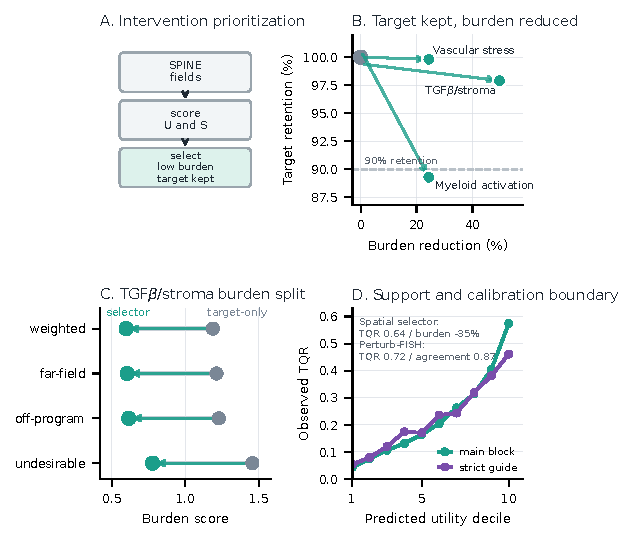
\includegraphics[width=\linewidth]{selector_application_main.pdf}
\caption{\textbf{Response-field-based perturbation prioritization.}
(a) Formal field-to-decision interface. (b--c) Exploratory post-hoc cases
illustrating how matched target utility can coexist with different spatial
burden. (d) Confirmatory evaluation on the fully separated
train/validation/test selector split: the selector preserves target-qualified
rate 0.6944 while reducing mean spillover by 12.0\%; absolute held-out burden
decreases by 0.1244 [0.0559, 0.1926]. The post-hoc cases are illustrative and
are not used as confirmatory effect estimates.}
\label{fig:selector_application_kdd}
\Description{Four-panel perturbation-prioritization figure showing the decision
interface, exploratory matched-utility cases, an exploratory burden
decomposition, and formal held-out selector estimates.}
\end{figure}

\begin{table}[t]
\centering
\scriptsize
\caption{\textbf{Formal three-way-split perturbation prioritization.} Train, validation, and test partitions are fully separated; target qualification is unchanged relative to target-only. Larger discovery-set reductions and biological examples are exploratory post-hoc analyses in the appendix.}
\label{tab:selector_main}
\setlength{\tabcolsep}{2.5pt}
\resizebox{\columnwidth}{!}{%
\begin{tabular}{lrrr}
\toprule
Method & TQR $\uparrow$ & Spill. red. $\uparrow$ & Abs. burden decrease $\uparrow$ \\
\midrule
Target-only & 0.6944 & 0.0000 & 0.0000 \\
Constrained selector & 0.6944 & 0.1200 & 0.1244 [0.0559, 0.1926] \\
\midrule
\multicolumn{4}{l}{\textit{Burden-ranking diagnostic}} \\
SPINE standalone spillover head & \multicolumn{3}{r}{0.6250 [0.6108, 0.6393]} \\
\bottomrule
\end{tabular}
}
\end{table}


On the fully separated selector split, the constrained selector preserves the
observed target-qualified rate of target-only (0.6944 versus 0.6944) while
reducing mean spillover by 12.0\%. Absolute burden decreases by 0.1244
[0.0559, 0.1926]. A standalone \methodname{} spillover head reaches pairwise
burden-order agreement 0.6250 [0.6108, 0.6393], supporting learnable ranking
signal. The effect is positive but moderate, and the observed-field oracle
shows substantial remaining room.

The previously reported 35.4\% aggregate reduction and the
TGF-$\beta$/stroma, vascular-stress, and myeloid-activation examples were
identified in the discovery analysis. We retain them only as exploratory
illustrations of the utility--burden mechanism and do not use them as
confirmatory effect estimates. Perturb-FISH calibration and module-level
support are likewise reported in the appendix.

\clearpage
\section{Discussion}
\label{sec:discussion_conclusion}
The principal finding is a decomposition of predictive signal. Tissue context
accounts for most global field structure, while perturbation conditioning adds
a smaller but reproducible radial component. Matching-decoupling and
profile/location controls narrow the interpretation further: expression
overlap alone does not explain the lift, spatially local pseudo-controls remain
necessary, and both the sender profile and its location matter. This resolves
the apparent tension between strong context reconstruction and non-zero
perturbation lift: they describe different estimands.

\methodname{} operationalizes this distinction with a frozen context predictor
and direct-effect-to-receiver residual routing. Its conditional guide-OOD
result supports reuse when an assay-matched spatial seed is available, but the
external scRNA failure shows that end-to-end perturbation transfer is not
solved. The formal selector converts the predicted field into a practical
experimental decision: among actions expected to meet a local objective, which
one has lower far-field and off-program burden? Its 12.0\% held-out reduction is
modest but credible, and motivates better direct-effect transfer and target
calibration rather than a more elaborate routing prior.

\section{Limitations and Ethical Considerations}
\label{sec:limitations_ethical_considerations}
\ppp remains a matched pseudo-counterfactual rather than an observed pre/post
measurement of the same cells. Positive lift survives gene-disjoint and
no-expression matching but disappears without spatial matching, so conclusions
depend on local control states. The reported cache collapses nominal coarse
cell-state labels to one mapped ID, preventing cell-type-stratified claims.
The 64-cell setting maximizes paired lift in this mouse-brain assay, but its
approximately 98\,$\mu$m scale may not transfer across tissues, platforms, or
cell densities. Guide-OOD gain from assay-matched spatial seeds is modest, and
companion scRNA seeds underperform zero seed. Cached communication scores and
the reference-ST adapter provide no robust measured gain and are not core
components. The formal selector effect is positive but moderate; larger
discovery-set reductions and individual biological cases are post-hoc
illustrations. No result has prospective spatial perturbation validation.

\methodname{} and its prioritization outputs are for experimental hypothesis
generation, not clinical decision making, treatment recommendation, or
therapeutic safety assessment. Public or de-identified molecular data can
retain sensitive tissue, disease, and donor information; reuse must follow
original consent, IRB, and data-use terms. Broader tissues and species,
prospective intervention tests, and domain-expert review are required before
acting on a prioritized perturbation.

\clearpage
\section{Generative AI Usage}
Generative AI tools assisted language editing and code development. The authors
independently checked all designs, results, figures, and interpretations. No
generative AI model constructed benchmark targets or experimental labels.

\section{Code and Data Availability}
\label{sec:code_release}
We will release code, configurations, split manifests, machine-readable source
tables, and evaluation scripts in a public repository; the archival URL will be
added before submission. All datasets are public and remain subject to their
original terms.

\section{Reproducibility Statement}
The submission bundle separates strict confirmatory, original exact-task, and
exploratory post-hoc results in a machine-readable claims registry. Tables
1--3 are generated from versioned CSV files rather than manually duplicated
values. The release will include spatial and grouped-guide split manifests,
model and selector configurations, bootstrap units, figure-generation scripts,
and result-provenance records that map each reported estimate to its source
file. Exact-task and strict-split results are stored separately to prevent
cross-split comparison.

\typeout{SPINE-MAIN-END-PAGE=\thepage}
\clearpage
\bibliographystyle{ACM-Reference-Format}
\bibliography{references}
